\documentclass[12pt]{article}%
\usepackage{amsmath,amssymb,amsthm,amsfonts}
\usepackage{wasysym}
\usepackage{graphicx}
\usepackage[dvipsnames]{xcolor}
\usepackage{stackengine}
\def\stackalignment{l}
\usepackage[colorlinks]{hyperref}
\usepackage{tikz}
\usepackage[export]{adjustbox}

%\usepackage{geometry}
%\geometry{top = 0.9in}
\usepackage{appendix}

\usepackage{commands}



\usepackage{caption}
\usepackage{subcaption}


\newcommand{\ea}{\textit{et al. }}
\renewcommand{\epsilon}{\varepsilon}
\renewcommand{\th}{\text{th}}
\newcommand{\sgn}{\operatorname{sgn}}

\renewcommand{\setminus}{\smallsetminus}

\newtheorem{thm}{Theorem}
\newtheorem{lemma}{Lemma}

\definecolor{red}{rgb}{0.8500, 0.3250, 0.0980}
\definecolor{green}{rgb}{0.4660, 0.6740, 0.1880}
\definecolor{yellow}{rgb}{0.9290, 0.6940, 0.1250}
\definecolor{blue}{rgb}{0, 0.4470, 0.7410}


\begin{document}

\title{Coding Project 3:  Principal Component Analysis of a Mass-on-a-spring System}

\author{Marvyn Bailly}
\date{February 24, 2023}

\maketitle


\begin{abstract}
In this coding project, we begin with a brief motivation behind the Principal Component Analysis and Mass-on-Spring systems. We continue to discuss elements of the mathematical theory behind, Singular Valued Decomposition, Rank-$n$ approximations, and Principal Component Analysis. Next we consider four experiments were the motion of a mass on a spring is measurement using three cameras. In each experiment, the data is subject to increasing levels of noise. We demonstrate how to numerically apply Principal Component Analysis on the dataset to approximate the position of the mass throughout time. We conclude by presenting the results and discussing the effectiveness of Principal Component Analysis. 
\end{abstract}


\section{Introduction}
\label{Sec: Intro}

Principal Component Analysis (PCA) is a widely used technique in data science and other various fields for analyzing large datasets. The PCA method is formally a statistical technique that reduces the dimensionality of a dataset while preserving the essential information. This is achieved by linearly transforming the data into a coordinate system where the features of the data can be described in fewer dimensions. PCA is used across many fields including image and signal processing, data mining, finance, and engineering. In finance, PCA is used to analyze and identify the key drivers of the stock market by reducing the number of variables to focus on. Another application of PCA is in data mining, where it is used to identify hidden patterns in the data by identifying the most significant variables. In mathematics, PCA can be applied to dynamical systems, to capture important features such as the motion of the mass, the energy distribution, and the frequency content of the system. An example of such a system, is the classic example of the oscillatory behavior of a mass-on-spring system.

Mass-on-spring systems, also known as spring-mass systems, are ubiquitous in mechanical engineering, mathematics, physics, and other scientific disciplines. An example of a spring-mass system is a mass suspended by a spring. In the ideal case, the mass is perturbed from its resting point, known as the equilibrium, only in the vertical direction. This causes the mass to oscillate up and down about the equilibrium until it comes to a rest at the equilibrium. The dynamics of this behavior can be described by the ordinary differential equation
\begin{equation} \label{oscillatory}
    \ddn{2}{f(t)}{t} = - \omega f(t),
\end{equation} 
where $f(t)$ measures the displacement of the mass as a function of time. The governing equation \fullref{oscillatory} has the well known solution
\begin{equation}
    f(t) = A \cos(\omega t + \omega_0),
\end{equation}
where $A$ and $\omega_0$ depend on the initial state of the system. In practice, data describing the motion of a spring-mass system are subject to noise such as unstable cameras and other external perturbations on the system that make its motion harmonic up to some asymptotic order of $\eps$. The PCA process can be applied to extract the key information about the system through the noise.   



\bigskip
\bigskip

In this coding project, we will explore the application of PCA on a mass-spring experiment with increasing amounts of noise in the data measurements. The PCA method will be used to track the position of the mass throughout time. We begin by explaining the mathematical theoretical background of Singular Value Decomposition, Rank-$n$ Approximations, and Principal Component Analysis. Next we will demonstrate the numerical methods of the mathematical concepts on four increasingly noisy mass-spring experiments to approximate the mass's position throughout time. Finally we will present and discuss the results from the numerical analyze before concluding with final thoughts on the PCA method and the experiments.  



\section{Theoretical Background}

In this section, we will explore the derivations and motivations of the Singular Value Decomposition, Rank-$n$ Approximations, and PCA. We will highlight the relations between the concepts and how they can be applied in combination to analyze data sets.   


\subsection{Singular Value Decomposition}

The Singular Value Decomposition (SVD) is a type of matrix factorization that decomposes a matrix into three component matrices, all of which contain important information about the original matrix depending on the application. The concept of the SVD is best understood geometrically. Consider a unit sphere in $\R^m$ and a matrix $A \in \R^{m \times k}$ where $m \geq k$ without loss of generality. The image of the unit ball under $A$ is a hyperellipse in $\R^m$ that is achieved by rotating and stretching the principal axes of the unit ball. The amount that each axes of the unit ball, call them $\mathbf{v}_1,\mathbf{v}_2,\dots,\mathbf{v}_k \in \R^k$ and note they are orthogonal, is stretched by some scalar quantity, $\sigma_1, \sigma_2, \dots, \sigma_m \in \R$ in the orthogonal directions $\mathbf{u}_1, \mathbf{u}_2, \dots, \mathbf{u}_m \in \R^m$. Thus $\sigma_j \mathbf{u}_j$ are the principal semiaxes of the hyperellipse in $\R^m$ while $\mathbf{v}_j$ describe the semiaxes of the original unit ball. Note that $k$ of the $\sigma_j$ values will be nonzero and that is common practice to order the values as $\sigma_1 \geq \sigma_2 \cdots \geq \sigma_k > 0$. Now we have that
\begin{equation}
    A \mathbf{v}_j = \sigma_j \mathbf{u}_j, ~~~~ 1 \leq j \leq k,
\end{equation}
for the nonzero $\sigma$ values. Combining the vectors $\mathbf{u}_j$ into a $m \times k$ matrix $\hat{U}$, the vectors $\mathbf{v}_j$ into a $k \times k$ matrix $V$ and the values $\sigma_j$ into a diagonal matrix $\hat{\Sigma}$, gives 
\begin{equation} 
    \begin{bmatrix}\label{lol}
        A
    \end{bmatrix} \begin{bmatrix}
        \mathbf{v}_1 & \mathbf{v}_2 & \cdots & \mathbf{v}_k
    \end{bmatrix} = \begin{bmatrix}
        \mathbf{u}_1 & \mathbf{u}_2 & \cdots & \mathbf{u}_k
    \end{bmatrix}  \begin{bmatrix}
        \sigma_{1} &  &  & \\ 
        & \sigma_{2} &  & \\ 
        &  &  \ddots & \\ 
        &  &   & \sigma_{k} 
      \end{bmatrix}.
\end{equation}
\fullref{lol} can be rewritten as
\begin{equation} \label{reduced SVD}
    A = \hat{U}\hat{\Sigma} V^{-1},
\end{equation}
which is known as the reduced SVD of $A$.

The columns of $\hat{U}$ are known as the left singular vectors of $A$ while the columns of $V$ are the right singular vectors of $A$. The diagonal entries of $\hat{\Sigma}$ are known as the singular values of $A$. Note that the idea of the SVD can be extended to complex matrices. To achieve the full SVD of a matrix, $m-k$ vectors that are orthogonal to the columns of $\hat{U}$ are added to $\hat{U}$ to get $U \in \C^{m \times m}$. To match the dimensions of the matrices, $m-k$ rows of zeros are added to the bottom of $\hat{\Sigma}$ to get $\Sigma \in \R^{m \times k}$ diagonal matrix. Thus we have the full SVD of $A$ to be
\begin{equation}\label{full svd}
    A = U \Sigma V^*,
\end{equation}  
where $U$ and $V$ are unitary matrices. The SVD plays a critical role in many applications as the decomposition can be used to solve linear systems and create low-rank approximations of matrices.   


\subsection{Rank-n Approximation}

To understand the idea behind Rank-$n$ approximations, we return to the geometric interpretation of the SVD. If the matrix $A$ is rank $r \leq k$, then there will be $r$ nonzero nonsingular values in the SVD and the unit ball is transformed into a $r$-dimensional hyperellipse. In this case, $A$ is fully captured and no information is lost since. But what if we want the best approximation of $A$ in the $r-1$th dimension? The solution is to take the first $r-1$ singular values from $\Sigma$ and similar the corresponding $r-1$ columns of $U$ and $V^*$, and compute the SVD of $A$ using these matrices. This will project the $r$ dimensional hyperellipse onto the $r-1$ plane. Recalling that we ordered $\sigma_1 \geq \cdots \geq \sigma_r$, the most information about the structure of $A$ is stored in $\sigma_1$ and the corresponding left and right singular values. Thus only a little amount of information is lost in the $r-1$th projection. Thus, if we want to find the best line segment to approximate the hyperellipse, we simply use the line segment formed by the major axes of the hyperellipse that is associated to $\sigma_1$.    

More formally, we reconsider the SVD of $A$ as the sum of $r$ rank-one matrices,
\begin{equation}
    A = \sum_{j =1}^{r} \sigma_j \mathbf{u}_j \mathbf{v}_j^*.    
\end{equation}
Now if we reduce the number of rank-one matrices used to compute $A$ to $0 \leq n \leq r$, we have 
\begin{equation} \label{rank n}
    A_n = \sum_{j = 1}^{n} \sigma_j \mathbf{u}_j \mathbf{v}_j^*,
\end{equation}
which is the Rank-$n$ approximation $A$. Therefore, we see that the SVD of a matrix can be used to project onto lower dimensions. The error of the Rank-$n$ approximation is given by
\begin{equation}
    e_n = \|A - A_n \|. 
\end{equation} 
In summary, the SVD provides a powerful tool for computing rank-n approximations of matrices, which can be used to capture the essential features of the data and reduce its dimensionality.

\subsection{Principal Component Analysis}

PCA is a mathematical technique for analyzing data and finding the directions in which the data varies the most. In practice, a dataset is highly susceptible to noise, redundant information, and suboptimal viewpoints. To remedy this, PCA uses methods to remove redundant and extract the dominant variance of the dataset. 

Given a dataset $\mathbf{X} \in \C^{m \times n}$ consisting of $m$ observations of $n$ variables, the goal of PCA is to find the principal components of $\mathbf{X}$. The first principal component $\mathbf{u}_1$ is the direction in which the data varies the most, and is given by the eigenvector corresponding to the largest eigenvalue of the covariance matrix $\mathbf{C}_\mathbf{X}$ of $\mathbf{X}$. Subsequent principal components $\mathbf{u}_2, \ldots, \mathbf{u}_m$ correspond to smaller variances but are ordered largest to smallest. The covariance matrix $\mathbf{C}_\mathbf{X}$ is defined as 
\begin{equation}
    \mathbf{C}_\mathbf{X}=\paren{\frac{1}{n-1}}\mathbf{X}\mathbf{X}^T,
\end{equation}
where $\mathbf{X}$ is centered by subtracting the mean of each column, $\frac{1}{n-1}$ is a normalization constant for the unbiased estimator $\mathbf{X}\mathbf{X}^T$. The covariance matrix is a real square, symmetric $m \times m$ matrix whose main diagonal elements represent variance within measurement sets while the off diagonal elements show the variance between measurement sets. To study the relationships in $\mathbf{X}$, we need to extract the information of the diagonal elements without changing the off diagonal elements as to not destroy the correlations in the data. One method to achieve this goal is to diagonalize $\mathbf{C}_\mathbf{X}$.  

Since $\mathbf{C}_\mathbf{X}$ is a real square, symmetric, and real, Linear algebra states that there exists an eigenvalue Decomposition of $\mathbf{X}\mathbf{X}^T$ of the form
\begin{equation}
    \mathbf{X}\mathbf{X}^T = \mathbf{S}\mathbf{\Lambda}\mathbf{S}^{-1},
\end{equation}
where the columns of $S$ are the eigenvectors of $\mathbf{X}\mathbf{X}^T$. This gives principal component basis
\begin{equation}
    \mathbf{Y} = \mathbf{S}^TX.
\end{equation}
In this basis, the eigenvectors of $\mathbf{X}\mathbf{X}^T$ are the principal components and the covariance can be found by 
\begin{equation}
    \mathbf{C}_\mathbf{Y} = \frac{1}{n-1}\mathbf{Y}\mathbf{Y}^T = \frac{1}{n-1}\mathbf{\Lambda}.
\end{equation}
Another approach to diagonalizing $\mathbf{C}_\mathbf{X}$ is using the SVD method. If we compute the SVD of $\mathbf{X}$ as $\mathbf{X} = \mathbf{U}\mathbf{\Sigma}\mathbf{V}^*$, then the principal component basis is given by 
\begin{equation}
    \mathbf{Y} = \mathbf{U}^*\mathbf{X},
\end{equation}
and the covariance is given by
\begin{equation}
    \mathbf{C}_\mathbf{Y} = \frac{1}{n-1}\mathbf{Y}\mathbf{Y}^T = \frac{1}{n-1}\mathbf{\Sigma}^2.
\end{equation}
Thus we can use the SVD method to find the principal components of $\mathbf{X}$ to be the columns of $\mathbf{U}$ and the variance are the diagonal elements of $\mathbf{\Sigma}^2$. Since we are using SVD, the covariance and principal components are already ordered from highest variance to lowest. 

\section{Numerical Methods}


We now extent the theoretical concepts to a mass-spring experiment. In the experiment, three cameras are used to record the motion of a mass on a spring. The mass is perturbed from the equilibrium and we assume that the oscillatory behavior is only in the $z$-plane. Since each camera is recording the position of the mass from a different angle, we can collect the data as following:
\begin{subequations}
    \begin{align}
        &\text{camera 1: } ~(\mathbf{x}_a, \mathbf{y}_a)\\
        &\text{camera 2: } ~(\mathbf{x}_b, \mathbf{y}_b)\\
        &\text{camera 3: } ~(\mathbf{x}_c, \mathbf{y}_c)
    \end{align}
\end{subequations}
where $a,b,$ and  $c$ are used to denote the camera and $(\mathbf{x}_j, \mathbf{y}_j)$ is the position of the mass over time in the $x-y$ plane of the camera. We note that the $x-y$ plane of the cameras may not exactly be the $x-y-z$ plane of the oscillating mass system. All the data is collected into a single matrix
\begin{equation} \label{big x}
    \mathbf{X} = \begin{bmatrix}
        \mathbf{x}_a\\
        \mathbf{y}_a\\
        \mathbf{x}_b\\
        \mathbf{y}_b\\
        \mathbf{x}_c\\
        \mathbf{y}_c
    \end{bmatrix}.
\end{equation}
Here $\mathbf{X}$ is a $6 \times n$ matrix where $n$ is the number of measurements taken by the camera. 

To analyze the motion of the mass-spring system, we use the PCA method which combines the ideas of the SVD method and Rank-$n$ approximations. Applying the SVD decomposition on the dataset $\mathbf{X}$, gives the principal components $\mathbf{U}$ and the variance of the data set $\mathbf{\Sigma}$. Next, we study the variance of the data to figure out which Rank-$n$ approximation will maintain the major behaviors of the data at the lowest cost. To do this we study the spectrum of singular values which is computed by
\begin{equation}\label{energy}
    \text{Energy} = \sum_{i,j = 1}^{n}\paren{\frac{1}{\mathbf{\Sigma}_{ij}}} \cdot \mathbf{\Sigma},
\end{equation} 
Plotting this values, shows the amount of variance between the singular values and thus allows us to make an appropriate choice for the Rank-$n$ approximation (further discussion in Results Section).

We preformed the numerical methods in MATLAB and use the same process for each experiment. We begin by making sure that the measurements $(\mathbf{x}_j, \mathbf{y}_j)$ taken by each camera is the same length. Next we center the data by subtracting the mean of the data. Then we form the data matrix $\mathbf{X}$ as shown in \fullref{big x}. Next we find the SVD of $\mathbf{X}$ using MATLAB's \verb+svd+ function with the 'econ' option which concatenates the SVD to remove zero valued singular values and their corresponding left and right vectors. Next we compute the energies of the singular values as shown in \fullref{energy}. Studying the energy on a log plot allows us to find an appropriate Rank-$n$ approximation to use. Finally we compute the Rank-$n$ approximation of the SVD, as shown in \fullref{rank n}, to get a lower dimensional approximation of the location of the mass throughout time.  


\section{Results}

In this section, we will explore the results of the numerical methods applied to each of the experiments.

\subsection{Test 1: Ideal Case}

\begin{figure}
    \begin{subfigure}[b]{0.5\linewidth}
      \centering
      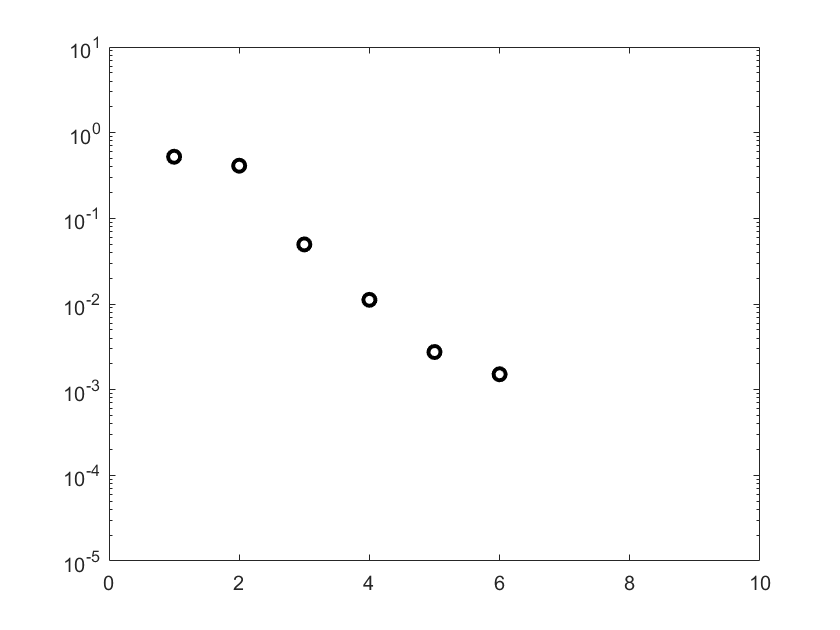
\includegraphics[width=\linewidth]{1-energy.png}
      \caption{Energy of Singular Values.}
      \label{fig1:a}
      \vspace{4ex}
    \end{subfigure}%%
    \begin{subfigure}[b]{0.5\linewidth}
      \centering
      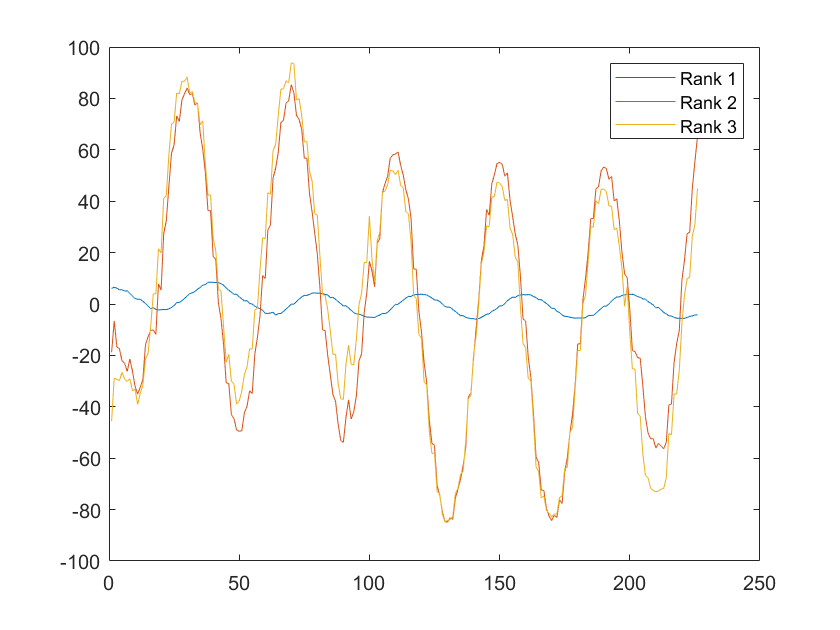
\includegraphics[width=\linewidth]{1-aprox.png}
      \caption{Plot of the Rank-$n$ approximations.}
      \label{fig1:b}
      \vspace{4ex}
    \end{subfigure}
    \caption{Plots used to determine and verify the appropriate Rank-$n$ approximate for the ideal case.}
    \label{fig1}
\end{figure}

In the first experiment, we have the ideal case were the cameras are not shaky and the mass is only perturbed in the $z$ plane. In this case, it is relatively easy for the cameras to track the oscillatory behavior of the mass. In Figure 1(a), we see the energies of the singular values plotted on a log plot. Clearly the first two singular values lay far above the others and thus we expect a rank-$2$ approximation to capture the defining details of the motion. Plotting the rank-$1$, rank-$2$, and rank-$3$ approximations of $\mathbf{X}$, as seen in Figure 1(b), using the SVD shows that a rank-$1$ matrix falls far short from the oscillatory motion seen in the rank-$2$ and rank-$3$ approximations. Comparing the rank-$2$ and rank-$3$ approximations we see that the rank-$2$ effectively captures the same information as the rank-$3$. The graph of the motion throughout time seems very reasonable to what we would expect. 





\subsection{Test 2: Noisy Case}

\begin{figure}
    \begin{subfigure}[b]{0.5\linewidth}
      \centering
      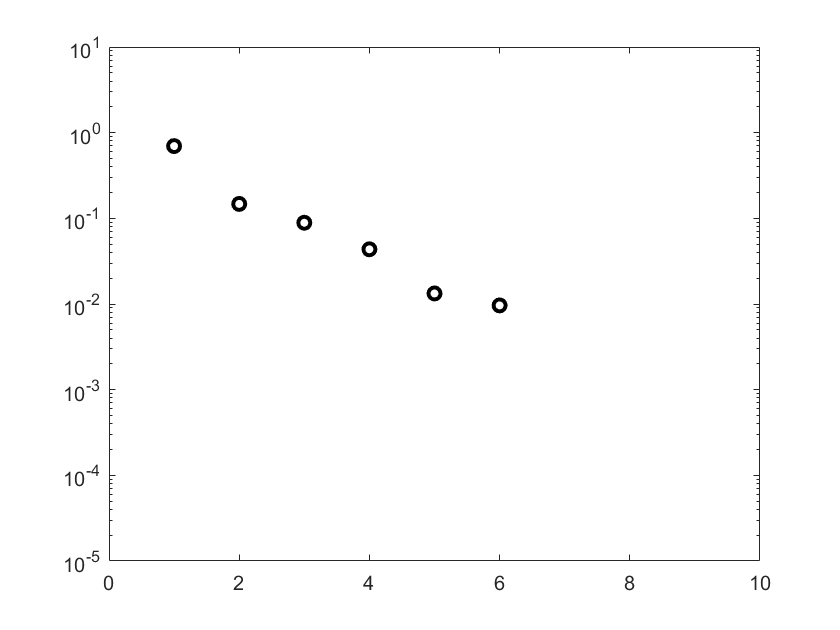
\includegraphics[width=\linewidth]{2-energy.png}
      \caption{Energy of Singular Values.}
      \label{fig2:a}
      \vspace{4ex}
    \end{subfigure}%%
    \begin{subfigure}[b]{0.5\linewidth}
      \centering
      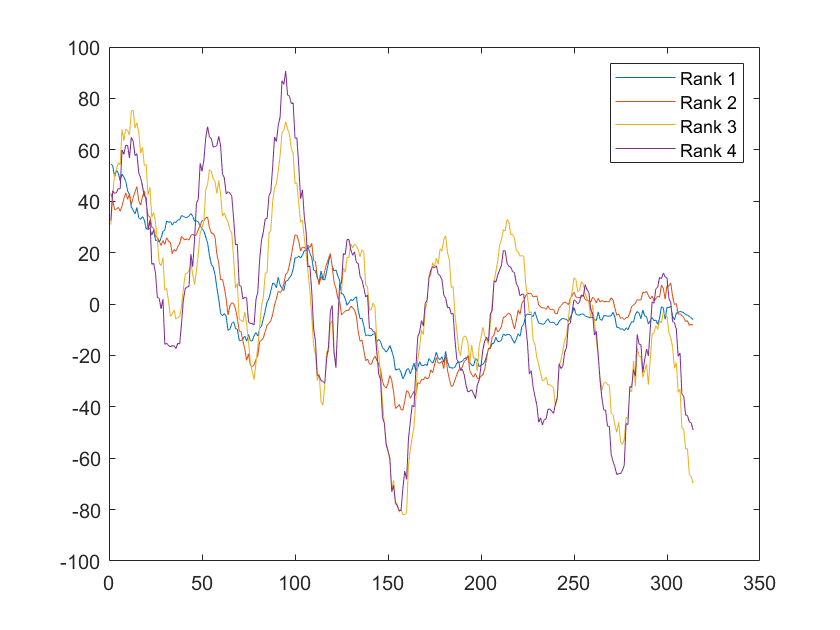
\includegraphics[width=\linewidth]{2-aprox.png}
      \caption{Plot of the Rank-$n$ approximations.}
      \label{fig2:b}
      \vspace{4ex}
    \end{subfigure}
    \caption{Plots used to determine and verify the appropriate Rank-$n$ approximate for the noisy case.}
    \label{fig2}
\end{figure}

In the second experiment, the mass is perturbed in the $z$ plane but now the cameras experience noise in the form of shaking. In this case, while the motion of the mass is easily observed to be oscillatory, it is more challenging to see the pattern through the shaky cameras. In Figure 2(a), we see the energies of the singular values plotted on a log plot. In this case it is more challenging to find the correct approximation to use. We see that the first singular value is above the others but the second, third, and fourth, are all close together. Plotting the rank-$1$, rank-$2$, rank-$3$, and rank-$4$ approximations of $\mathbf{X}$, as seen in Figure 2(b), shows that the rank-$1$ and $2$ approximations capture the correct motion but fail to gather reasonable amplitudes of the motion. On the other hand, the rank-$3$ and $4$ approximations do a considerably better job at capturing the oscillations and amplitude of the motion and since the rank-$3$ matrix does not greatly differ from the rank-$4$ matrix, it is reasonable to say that the rank-$3$ matrix is the best low-rank approximation of $\mathbf{X}$. In this case, the graph of motion seems less reasonable since we should expect motion similar to the first case. This being said, it is notable that the oscillatory behavior can still be observed in the data despite the noise. 

\subsection{Test 3: Off Center}

\begin{figure}
    \begin{subfigure}[b]{0.5\linewidth}
      \centering
      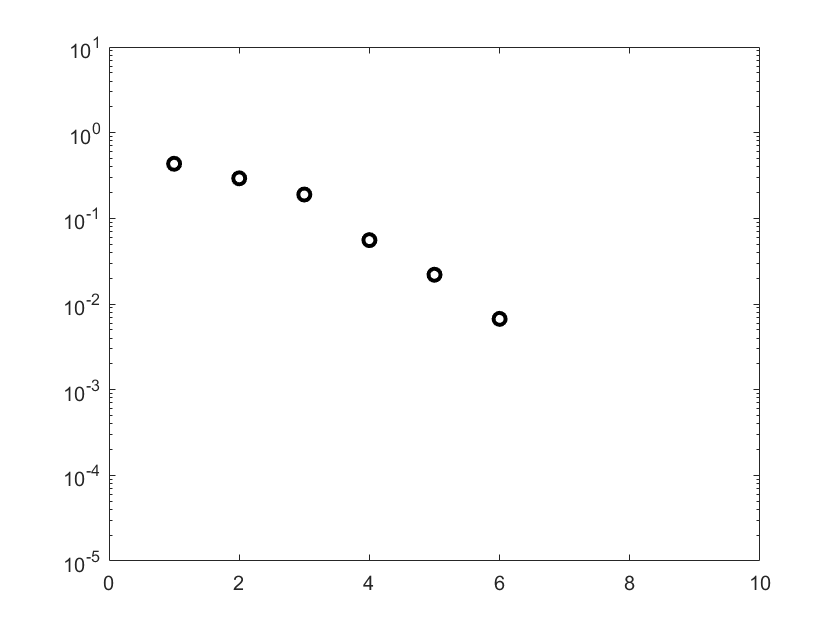
\includegraphics[width=\linewidth]{3-energy.png}
      \caption{Energy of Singular Values.}
      \label{fig3:a}
      \vspace{4ex}
    \end{subfigure}%%
    \begin{subfigure}[b]{0.5\linewidth}
      \centering
      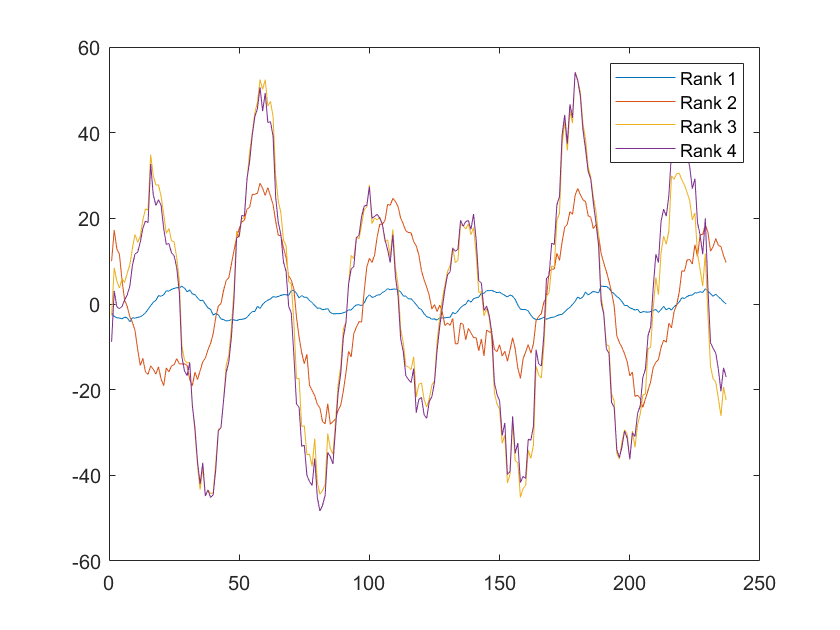
\includegraphics[width=\linewidth]{3-aprox.png}
      \caption{Plot of the Rank-$n$ approximations.}
      \label{fig3:b}
      \vspace{4ex}
    \end{subfigure}
    \caption{Plots used to determine and verify the appropriate Rank-$n$ approximate for the off center case.}
    \label{fig3}
\end{figure}

In the third experiment the cameras are steady again but the mass is perturbed not only in the $z$ plane but also in the $x$ and $y$. In this case, the motion of the mass is more complex than simple harmonic motion in the $z$ plane but we still expect harmonic motion up to some asymptotic order of $\eps$. In Figure 3(a), we see the energies of the singular values plotted on a log plot. In this case it is more challenging to find the correct approximation to use. We see that the first, second, and third singular values are above the others but it not immediately clear if a rank-$2$ approximation will suffice over a rank-$3$. Plotting the rank-$1$, rank-$2$, rank-$3$, and rank-$4$ approximations of $\mathbf{X}$, as seen in Figure 3(b), shows that the rank-$1$ approximation capture the correct motion but fails to gather reasonable amplitudes of the motion. In this case, the rank-$2$ approximation has significant error in certain times when compared to higher order approximations. On the other hand, the rank-$3$ and $4$ approximations do a considerably better job at capturing the oscillations and amplitude of the motion and since the rank-$3$ matrix does not greatly differ from the rank-$4$ matrix, it is reasonable to say that the rank-$3$ matrix is the best low-rank approximation of $\mathbf{X}$. In this case, the graph of motion seems reasonable since we should expect oscillatory motion similar to the first case. 


\subsection{Test 4: Rotation}

\begin{figure}
    \begin{subfigure}[b]{0.5\linewidth}
      \centering
      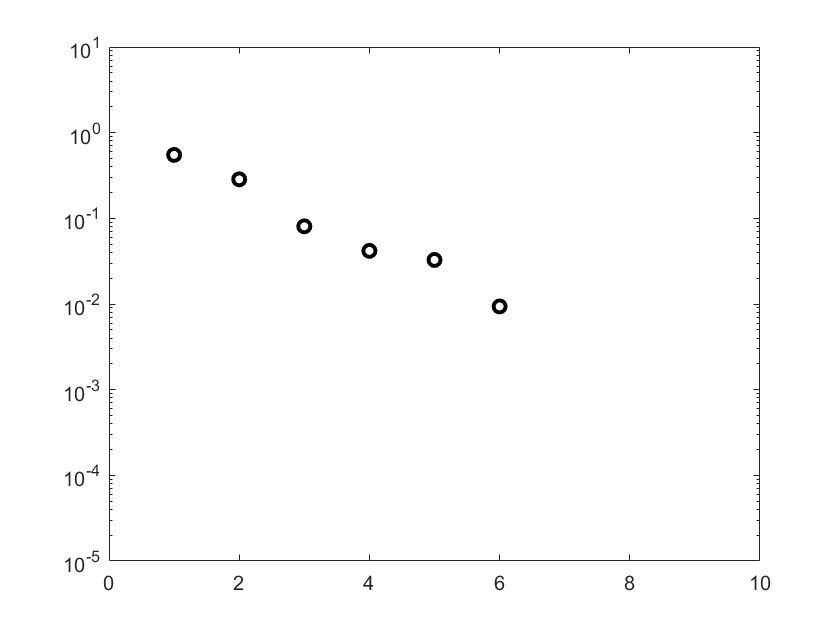
\includegraphics[width=\linewidth]{4-energy.png}
      \caption{Energy of Singular Values.}
      \label{fig4:a}
      \vspace{4ex}
    \end{subfigure}%%
    \begin{subfigure}[b]{0.5\linewidth}
      \centering
      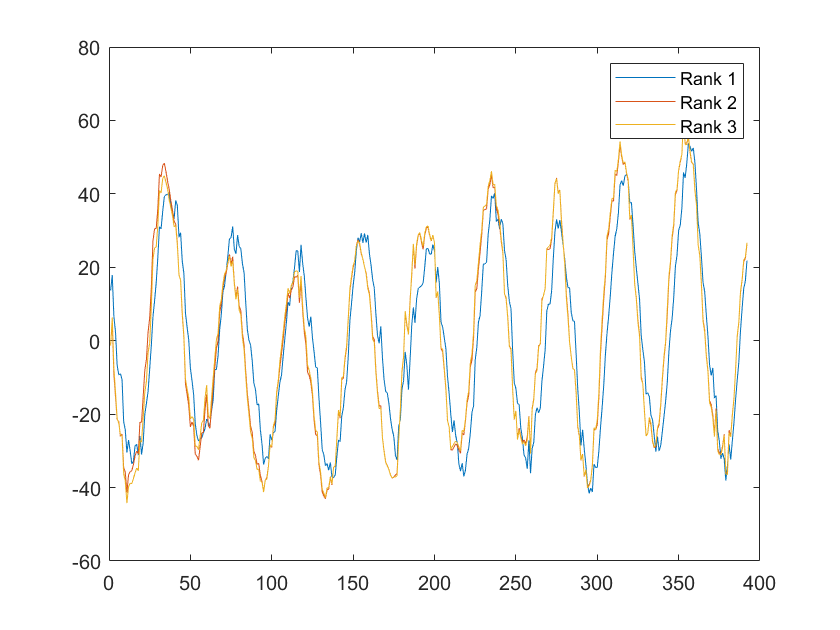
\includegraphics[width=\linewidth]{4-aprox.png}
      \caption{Plot of the Rank-$n$ approximations.}
      \label{fig4:b}
      \vspace{4ex}
    \end{subfigure}
    \caption{Plots used to determine and verify the appropriate Rank-$n$ approximate for the rotation case.}
    \label{fig4}
\end{figure}

In the final experiment, the mass is perturbed in a rotary motion and additionally, the cameras experience some noise in the form of shaking. In this case, we expect it to be challenging to pick out the oscillatory motion. In Figure 4(a), we see the energies of the singular values plotted on a log plot. In this case it is clear that the first and second singular values lay far above the others. Thus we can expect a rank-$2$ approximation to capture a reasonable amount of the variance. Plotting the rank-$1$, rank-$2$, and rank-$3$ approximations of $\mathbf{X}$, as seen in Figure 4(b), shows that the rank-$1$, $2$, and $3$ approximations are fairly similar. They all show similar oscillatory motion and the amplitudes across approximations stay consistent. In this case, we picked the rank-$2$ approximation to be the best as the rank-$2$ and $3$ approximations match each other closely while the rank-$1$ approximation falls slightly short. The graph of motion seems reasonable since we should expect oscillatory motion similar to the first case.


\section{Conclusion}\label{Sec: Conclusion}

In summary, for this coding project, we briefly discussed the applications and history of PCA and the mass-on-spring system. We further discussed the derivation and geometric meaning of the SVD method applied to matrices. We continued to show the relation between SVD and Rank-$n$ approximations of matrices. From here, the mathematical concepts and goals behind the PCA technique were examined. Next we explored the numerical method applications of PCA, SVD, and Rank-$n$ approximations on a dataset gathered from a mass-on-spring system. Finally we presented the results of the numerical methods applied to four experiments with increasing levels of noise introduced to the dataset. 

We end the report with some final thoughts on the PCA process and the effectiveness of this coding project. Firstly, we found it impressive how effective the PCA method is at identifying the motion of the mass despite noise. We were surprised that the second experiment seemed to be the most challenging to approximate with low-rank matrices. In the fourth case, we believe that a Rank-$1$ approximation suffices to capture the details of the motion. Overall we found this coding project to be insightful and interesting to further our understanding of the PCA method. 


\section*{Acknowledgment}

A special thanks to Alex Johnson, Charbel Younes, and Kaitlynn Lily who I worked with while coding the numerical methods. I would also like to thank my great friend and esteemed colleague Ike Griss for \LaTeX  and Visual Studio Code support :)





\end{document}
